\documentclass{article}

% Language setting
% Replace `english' with e.g. `spanish' to change the document language
\usepackage[danish]{babel}
% Set page size and margins
% Replace `letterpaper' with `a4paper' for UK/EU standard size
\usepackage[a4paper,top=2cm,bottom=2cm,left=3cm,right=3cm,marginparwidth=1.75cm]{geometry}

% Useful packages
\usepackage{amsmath}
\usepackage{graphicx}
\usepackage[colorlinks=true, allcolors=blue]{hyperref}
\usepackage{array}
\usepackage{subfig}
\usepackage{subfigure}
\usepackage{titlesec}
\usepackage{enumitem}

\title{CDIO delopgave 0}
\author{Jakob Agergaard}
\linespread{1.25}


\begin{document}

\titlespacing{\section}
    {0pt}{2em}{1em}




\begin{titlepage}
\begin{center}

    
\includegraphics[width=0.25\textwidth]{Billeder/DTULogo.png} \\
    \vspace{0.5cm}
    \Large
    \textbf{02314\hspace{1cm}62531\hspace{1cm}62532} \\
    Indledende programmering, Udviklingsmetoder til IT-systemer og Versionsstyring og testmetoder
    \vspace{0.4cm}
    \hrule
    
    \vspace*{0.5cm}
    \huge
    \textbf{CDIO delopgave 0}\\
    \LARGE
    Gruppe 17
    \vspace{0.5cm}
    \hrule
    \vspace{0.2cm}

    \large
    \begin{tabular}{m{10em} m{8em} m{8em} m{10em}}
    Jakob Skov Agergaard\vfill s224570 & 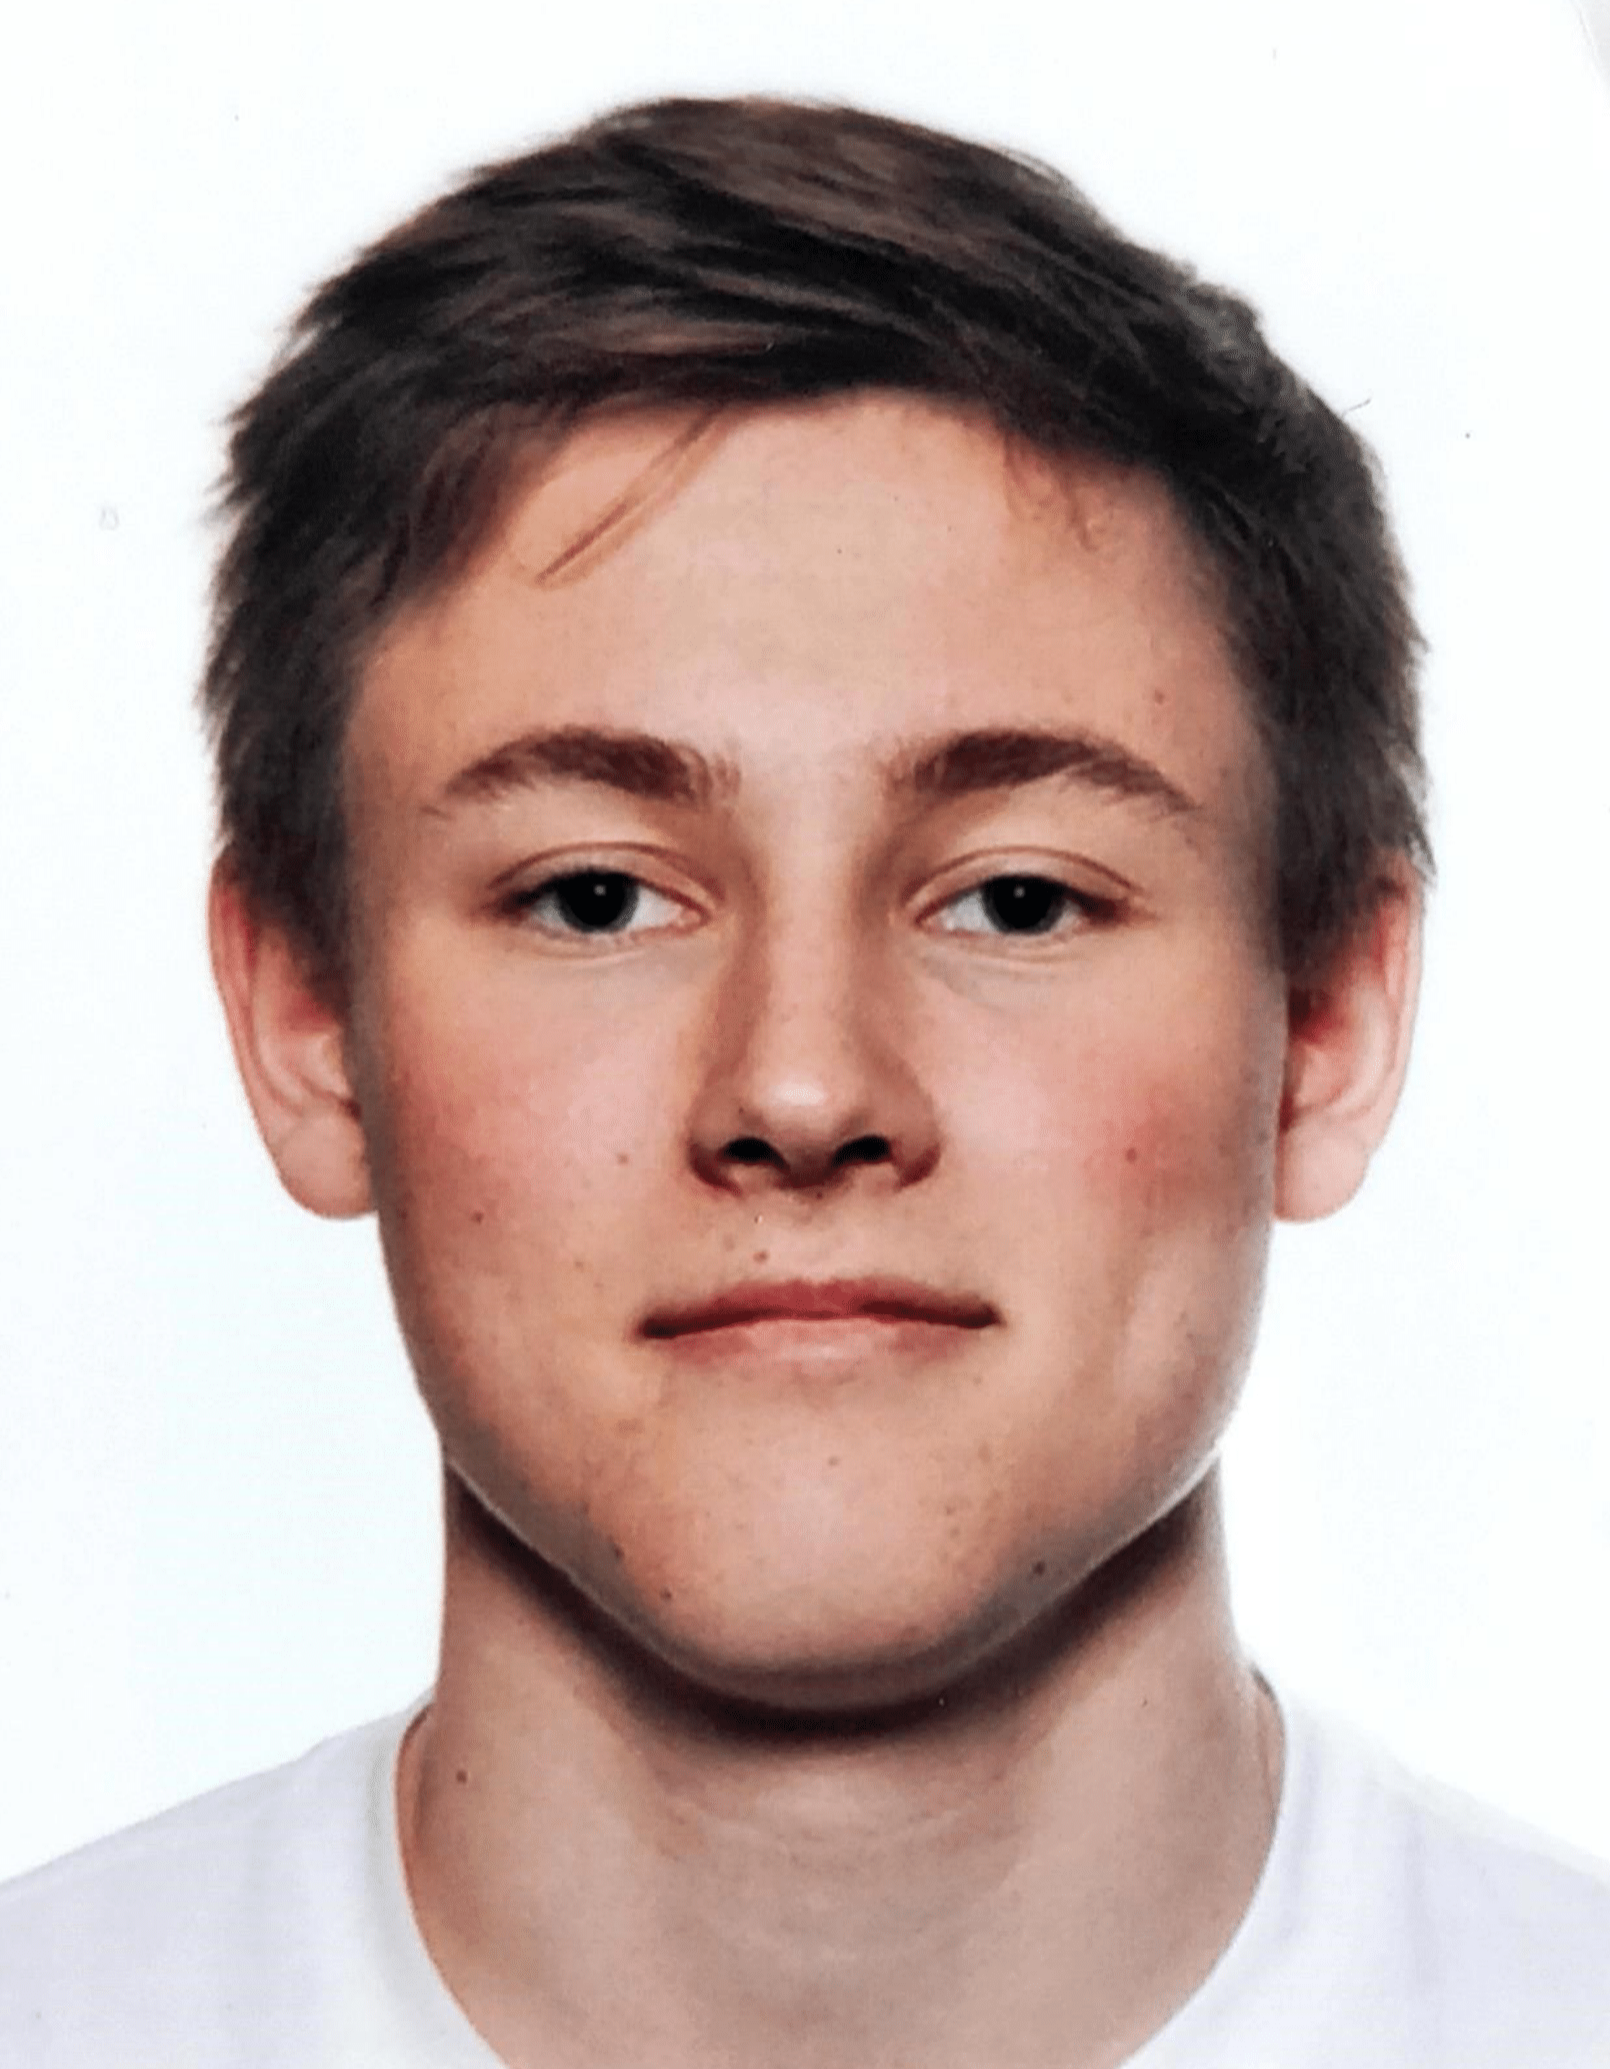
\includegraphics[width=0.2\textwidth]{Billeder/JakobFoto.png} & 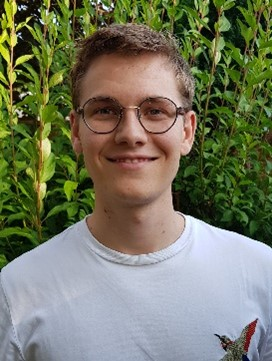
\includegraphics[width=0.2\textwidth]{Billeder/PhilipFoto.jpg} & Philip Muff Førrisdahl\vfill s224566 \\
    Mads Fogelberg Hansen\vfill s224563 & 
\includegraphics[width=0.2\textwidth]{Billeder/FotoMads.jpg} & 
\includegraphics[width=0.2\textwidth]{Billeder/EsbenFoto.png} & Esben Skovmand Elnegaard \vfill s224555  \\
    Jarl Boyd Roest\vfill s224556 & 
\includegraphics[width=0.2\textwidth]{Billeder/JarlFoto.png}
    \end{tabular}

    \vfill
    
    
    \vspace{1cm}
    \LARGE
    18. september 2022

    \vspace{1cm}
    
\end{center}
\end{titlepage}


\normalsize
\begin{abstract}
Der er på baggrund af kundens vision og krav er der blevet udviklet et Monopoly Junior spil. Efter kundens vision og krav var der egentligt rig mulighed for at forme sit Monopoly Junior spil efter eget ønske. En analyse er blevet lavet, hvor der er blevet produceret en række diagrammer, som har været hele forarbejdet til hele dette projekt. Der er også blevet lavet en bruger venlig test samt nogle test cases. Test casene illustrer de problemer, som projektet har stødt på, og den bruger venlige test er blevet lavet af unge mennesker som bor på kollegie, for at vise at mennesker, som ikke er en del af dette projekt eller ligende også kan spille det programmeret spil. Afslutningsvis kan det blevet konkluderet at spillet fungere som det skal, og at det kan spilles af andre mennesker som ikke er en del af dette projekt.
\end{abstract}
\break 

\tableofcontents
\break 

\section{Timeregnskab}

\section{Indledning}
I følgende rapport bliver hele handlings forløbet af vores CDIO-3 projekt beskrevet, samt dokumentation af denne proces. Rapporten giver kendskab til udviklingsmetoderne, som er brugt i processen. Projektet tager udgangspunkt i i børne spillet Monopoly Junior, men med mulighed for at implementere eller tilføje relevante ting. Der har været fokus på at bruge Rational Unified Process, som derfor har ført til små iterationer, evalueringer og opsamlinger under hele forløbet, både på forarbejdet og under programmerings delen, for hele tiden at sikre os at programmet køre som det skulle. Derudover er der blevet produceret en række diagrammer, som har overskuelig gjort opgaven, og dermed også nemmere at gå til. Der har været fokus på at bruge Low Coupling og High Cohesion til at lave diagrammeren. Dette kan ses da der har været fokus på nedarvning i diagrammerne, så klasserne arver metoder og variabler fra hianden. 

\section{Projekt-planlægning}
\begin{itemize}
    \item [1/11] Her laver vi en smule opgaveprioritering og udarbejder en hurtig kravsliste over funktionelle krav.\\
    Evaluering på dagen: Alt nået
    \item [2/11] Lave en primær use case beskrivelse (brief) og identificere andre sub-use cases. Udarbejde et use case diagram og starte på domænemodel.\\
    Evaluering på dagen: Alt nået, samt domænemodel færdiggjort og start på designklasse diagrammet. Vi har implementeret de første og simpleste klasser i IntelliJ.
    \item [4/11] Denne dag skal der laves system sekvensdiagram samt sekvensdiagram.
    \item [7/11]
    Afklaring af hvilke regler vi vil implementere og hvilke vi vil udelade, udover dem fra vores kravspecifikation. Design og test af boardclass og squareclass.
    \item [11/11]
    Opgaver for denne session:
    Færdiggjort strukturen af vores domæne/klassediagram. Få oprettet alle klasser samt toString metoder, samt toString metode til array. Oprettet og begynde små test i game class. Alt nået.
    
    \item [14/11]
    Opgaver løst: GUI implementeret. game funktionalitet implementeret og  første version af spillet færdigt. 
    Opgaver til næste gang: Implementere chancekort. Beskrivelse (output til spilleren) til felter og actions. Identificere Test og test cases.
    
    \item[15/11]
            Gennemgang af hvad programmet mangler, hvilke opgaver der skal løses og i hvilken rækkefølge,  og uddelegering af opgaver til enkeltmand.
            *Insert billede af tavle*
            
    \item[18/11]
            Folk laver tildelte opgaver, og en opsamling til sidst. 
            *refererer til billede af tavle*.
           
            Opsamling: Opgaver ikke nået; Junittest, gui-implementation af chancekort. Ansvarlige færdiggører s i weekend inden næste session.
                      
    \item [18/11]
    Bugs identificerede:
    Betaler først rent til den modtagen spiller runden efter.
    Køber ikke felt man lander på efter man har trukket chancekort
    Efter man har trukket et chancekort og lander på strandpromenaden, køber man ikke feltet. 
    Mulig problem løsning OG testcase: chancekortene kører kun 'set-loaction' metoden men ikke 'addlocation' metoden hvilket gør at spillerne ikke modtager penge når de har været i forbindelse med et chancekort
    \item [22/11]
    Sidste bugs vi har identificeret er løst, flere er dog identificerede men givet tiden givet til rådighed, vælger vi at lav code-freeze og fokusere på færdiggørelsen af rapporten. Den blvier skrevet færdig d. 25/11.
\end{itemize}
			efter vi har lavet vores design klasse diagram vil starte med at lave den klasse der har færrest bindinger til de andre 

		 \item[21/11]
            Gennemgang af de tildelte opgave, og videre arbejde af dem, hvis der er mangler. 

		
\section{Krav/Analyse}
\subsection{Kravsliste | funktionelle krav}
\begin{enumerate}
    \item Skal kunne spilles af 2-4 spillere
    \item Spilleplade med 24 felter
    \item Man skal kunne købe og derefter eje felter
    \item Spillerne skal have hver deres pengebeholdning
    \item Hvis én pengebeholdning går i minus slutter spillet
    \item En terning med seks sider
    \item En brik per spiller, som kan rykke
    \item 
\end{enumerate}
\subsection{Prioritering af krav vi vil implementere, når de funktionelle krav er opfyldt}
\begin {itemize}
\item Vi implementerer 3 af chancekortenes funktioner. Hvis der er tid implementere vi flere slags chancekort.
\item Fængsel felt og funktion bliver ikke implementeret. I stedet bliver de felter 'NonactionsFields'
\item Man får ikke mulighed for at vælge bil/farve men får blot tildelt en i starten af spillet.
\item  Spilstarteren bliver  den spiller der først indtaster sit navn
\item Spillerne starter med et tilpasset antal schmoney alt efter antal spillere
\item Spillere modtager penge ved landing eller passering af 'Start'-felt
\item hvis spilleren lander på et ledigt ejendeomsfelt, skal spillere købe det. Hvis spilleren lander på sit eget feldt skal spilleren ikke gøre noget. Dobbelt-ejendomsfelt reglen er udeladt.
\item Hvis spilleren lander på en andens ejendomsfelt, skal spilleren betale husleje.
\item Hvis 2 spillere har ens cash, i slutningen af spillet bliver værdien af deres ejedoms også sammentalt for at finde en endelig vinder.
\end {itemize}
\subsection{Use case beskrivelse }
\textbf{Scope:} Spil Monopoly Junoir  
\\
\textbf{Level:}
\\
\textbf{Primary actor:} Spillere 2 - 4 
\\
\textbf{Stakeholders and interests:} 
\item Spillerne vil spille et underholdende spil med formål at vinde. 
\item Projektvejlederen vil have et Monopoly Junoir spil, som vil tilfredsstille kundens vision og krav
\item Kunden vil have et monopoly spil, som har taget udgangspunkt i den fremlagte vision og de dertil hørende Monopoly Junoir regler 
\\
\textbf{Preconditions:} Computeren, som skal køre Monopoly Junoir skal have den nyeste version af Java. 
\\
\textbf{Succes guarantee:} Når en spiller går fallit tæller man sammen og finder en vinder 

\textbf{Sub use cases (beskrevet på 'brief format'):}
\begin{itemize}
    \item Ryk brik
    \item Vælg spillere
    \item Slå terninger
    \item Ændre pengebeholdning
    \item Skift tur
    \item Køb felt
\end{itemize}

\textbf{Use case skrevet på 'fully dressed' format:}\\


\textbf{Main Scenario}
\begin{enumerate}
\itemsep-0.5em
    \item Første spiller slår med terningerne
    \item Systemet lægger øjnene på terningerne sammen.
    \item Første spillers brik bliver nu rykket det antal felter som terningernes øjne viser.
    \item Spilleren lander på et felt og systemet fortæller hvilket felt man er landet på.
    \item Systemet fortæller hvilken handling eller hvad feltet gør\\
    \textit{Punkterne 1-5 bliver nu gentaget for næste spiller}
\end{enumerate}

\textbf{Main Succes Scenario}
\begin{enumerate}
\itemsep-0.5em
    \item Spilleren har slået med terningerne, rykket sine brikker og evt. købt/betalt/fået beløb, og turen er gået videre til næste spiller. 
\end{enumerate}
\textbf{Extension (Alternate Succes Scenario): }
\begin{enumerate}
    \item [4.a] Spilleren lander p̊a en grund der ikke er købt endnu. Systemet fortæller spilleren hvilket felt de er landet på. Spilleren har dog ikke nok penge til at betale feltets pris.
    \subitem 1. Spillet slutter da en spiller er gået fallit. Alle spillernes pengebeholdning bliver talt op, og den med flest penge vinder.
    \item [4.b] Spilleren lander på en grund der er købt. System fortæller spilleren hvilket felt de er landet på, og spilleren betaler samtidig husleje til spilleren som ejer feltet.
    \item [4.c] Spilleren lander på et felt uden handling.
\end{enumerate}

\section{Design}
Med henblik på at skabe det mest optimale Monopoly Junior, er der blevet fremstillet en række diagrammer, med formål at gøre opgaven mere overskuelig og dermed også nemmere. Det har været med fokus 	at bruge Low Coupling og High Cohesion til at lave diagrammerne.
\\

\begin{figure} [h]
    \centering
    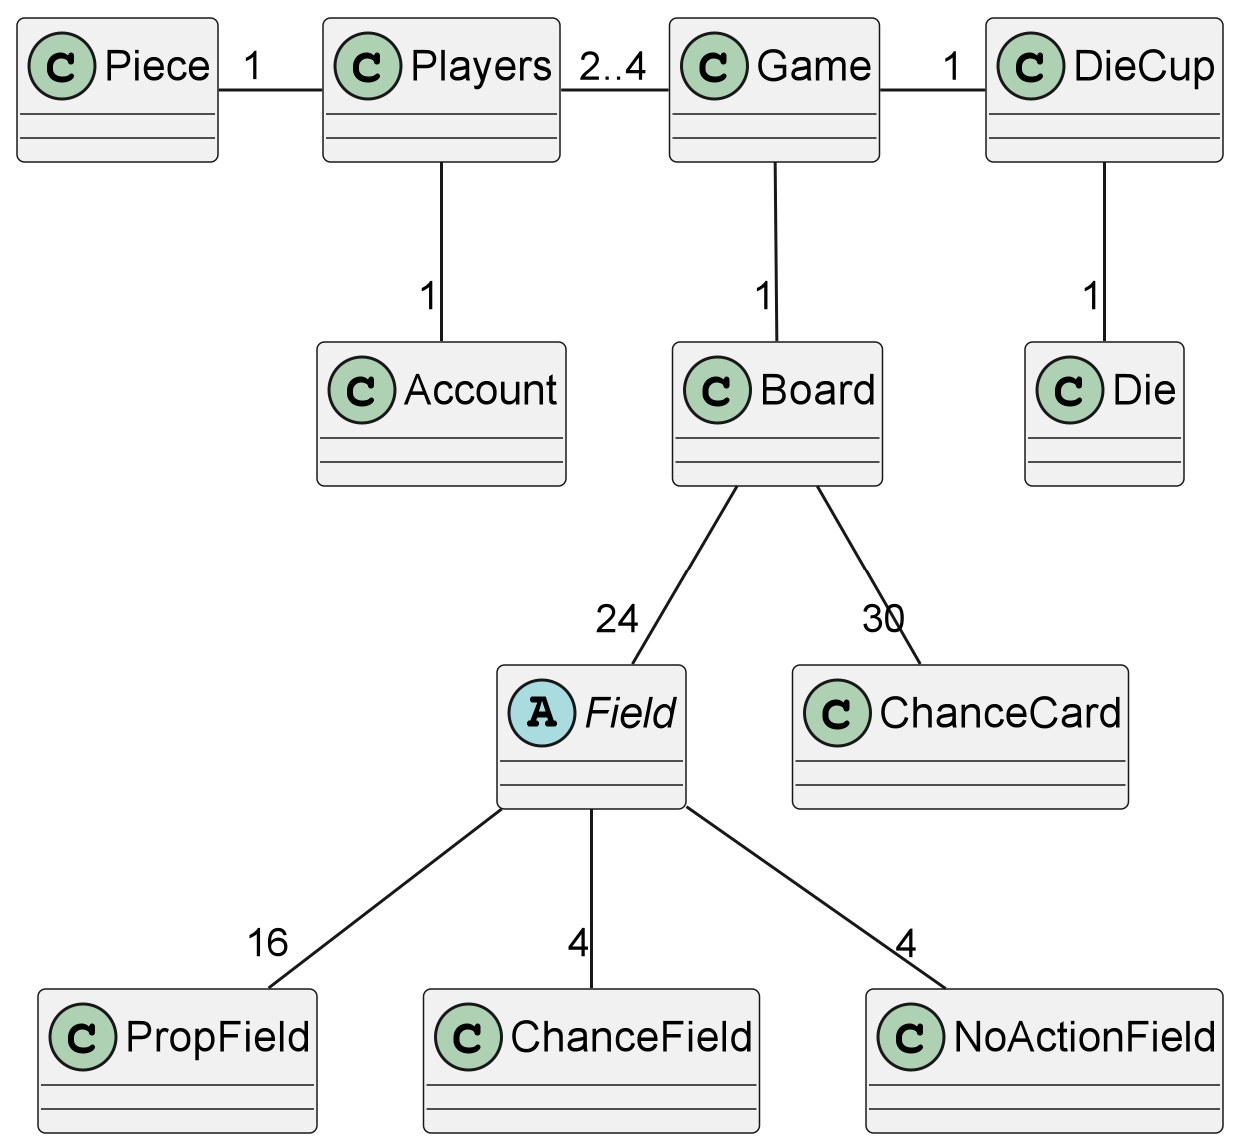
\includegraphics[width = 0.4\textwidth]{Billeder/Domænemodel.png}
    \caption{Domænemodel}
    \label{Domænemodel}
\end{figure}
Vores domæne model(Figur 1) er centralisereret omkring klassen game. Game klasen centralisereret programmet omkring game, da det giver mening at give en klasse som skal holde de andre. Man kan se at ud fra klassen Game, hvilke rolle de forskellige klasser har og hvordan de er bundet sammen. Der er hermed blevet brugt Low Coupling og High Cohesion, hvor der blevet gjort at hver enkel klasse er uafhængige som de kan være.  Klassen Field er blevet gjort til en abstract klasse, fordi klasserne Property-, Chance- og NoAntionField alle arve det samme fra Field klassen. Det er derfor smart at gøre dette til en abstract klasse, da det igen giver en bedre Low Coupling.
\\


\begin{figure} [h]
    \centering
    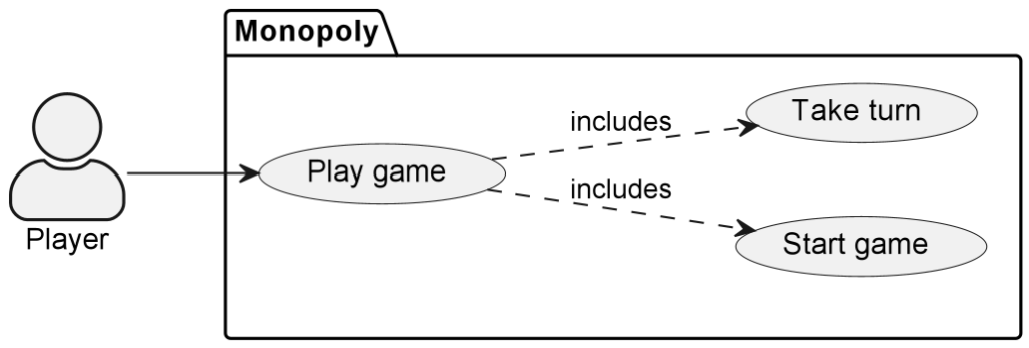
\includegraphics[width = 0.4\textwidth]{Billeder/Usecasediagram.png}
    \caption{Use case diagram}
    \label{Use case diagram}
\end{figure}
Dette use case diagram(Figur 2) viser hvordan spilleren og systemet interagere med hinanden. Spiller skal starte spillet og derefter starte turen, hvorefter spillet køre mere eller mindre ad sig selv. 
\\

\begin{figure} [h]
    \centering
    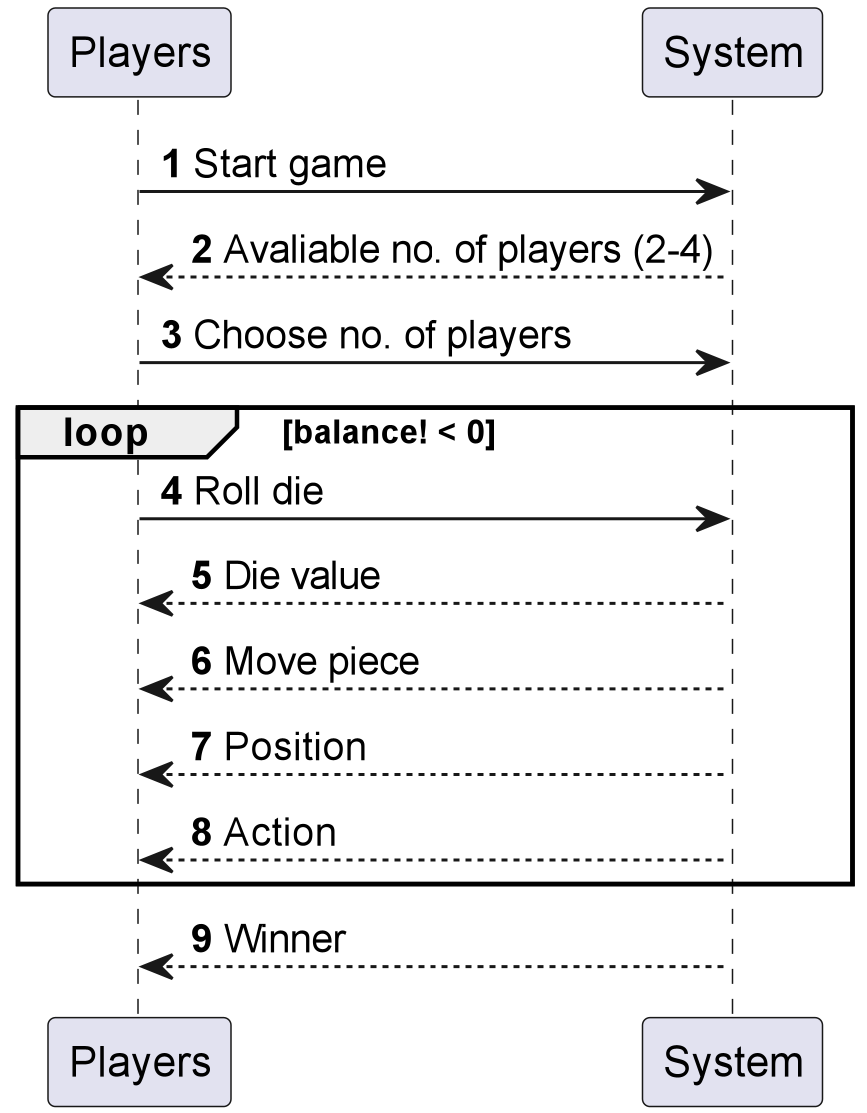
\includegraphics[width = 0.4\textwidth]{Billeder/Systemsekvensdiagram.png}
    \caption{System sekvens diagram}
    \label{System sekvens diagram}
\end{figure}
Vores system sekvens diagramFigur 3) illustrere, hvordan vores Monopoly Junior kommer til at forløbe sig overordnet. Diagrammet viser hvordan en sekvens af bedskeder går frem og tilbage over tid fra Players til System og fra System til Players. Diagrammet illustrere at man kun skal starte spillet, vælge antal spillere og slå terning, resten gør system, som giver bedskeder tilbage til spilleren om hvad man har slået, hvor man rykker hen og hvad feltet man lander på gør.     
\\

\begin{figure} [h]
    \centering
    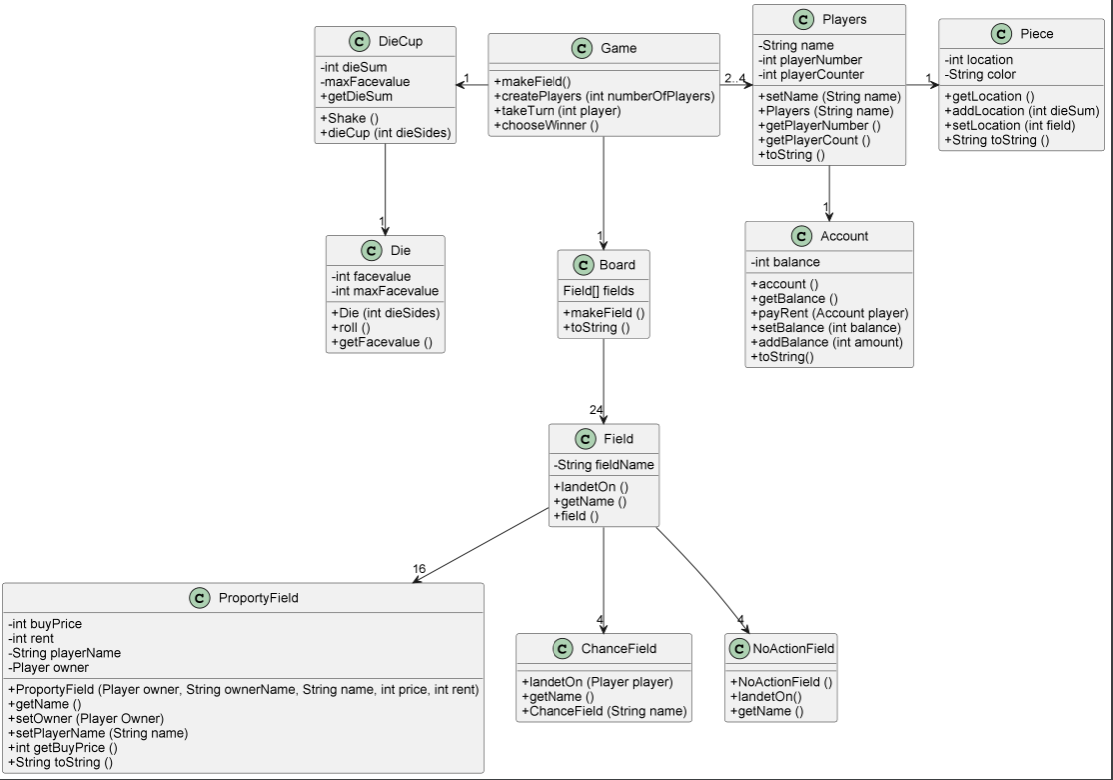
\includegraphics[width = 1.0\textwidth]{Billeder/Designklassediagram.png}
    \caption{Design klasse diagram}
    \label{Design klasse diagram}
\end{figure}
Design klasse diagrammet (Figur 4) visualisere klasse diagrammet mere specifikt, som er unikt for præcist denne opgave. Den giver en præcision af hvilke metoder og variabler, der har været tænkt der skulle bruges, og hvordan de enkel klasser arver fra hinanden. Klassen Piece ansvaret for lokationen af hver spillers brik på spille plade. Klassen Piece er information expert for lokation. Piece har ansvaret for lokationen da vi mener at det er her det giver bedst mening. Klassen Field har  to metoder landetOn og getName, som de dertilhørende klasser arver. Property-, Chance- og NoActionField arver alle denne metode, så det er derfor smart at ligge metoden oppe i klassen Field. 
\\
\\
\begin{figure} [h]
    \centering
    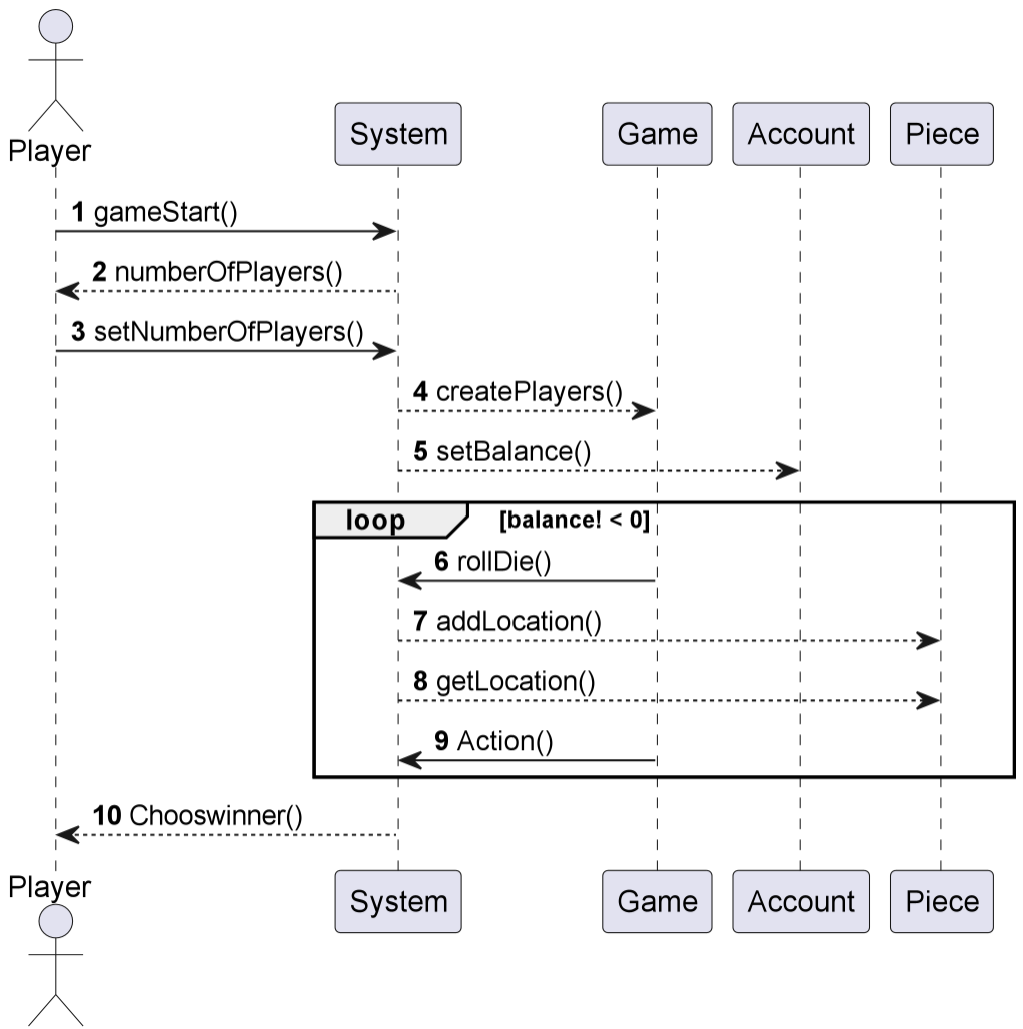
\includegraphics[width = 0.4\textwidth]{Billeder/designsekvensdiagram.png}
    \caption{Design sekvens diagram}
    \label{Design sekvens diagram}
\end{figure}
Dette design skevens diagram(Figur 5) viser, hvordan og i hvilken rækkefølge de forskellige klasser snakker sammen. Det kan ses at en  spillers balance bliver givet til en klasse Account, som holder styr på dette. Derudover kan det også ses at alle Locations metoderne bliver udført i klasse Piece. Design sekvens diagrammet giver et godt billede på hele processen i programmet fra start til slut på et grundlæggende niveau, så det er nemt at forstå for kunden. 
\\
\\

Når man bruger objekt orienterede programmering, som der bliver gjort i dette projekt, er det vigtigt at klasserne arver fra hinanden. En subklasse arver attributter og metoder fra en anden klasse, som hermed bliver til en superklasse. Man vil derfor lave et klasse hierarki, hvor subklasserne arver fra superklasserne. 
\\
\\
En abstrakt klasse er en superklasse, hvor alle de der tilhørende subklasser arver alt fra superklassen. Den abstrakte klasse kan ikke instansieres. 

\break
\section{Implementering}

\section{Test}
\subsection{Test case 01}
\begin{tabular}{ | m{0.2\textwidth} | m{0.8\textwidth}|}
    \hline
    Test case ID & TC01  \\
    \hline
    Summary & Tester at det rigtige antal spillere er indlæst fra brugeren, oprettet i spillet, oprettet som brikker, oprettet som pengebeholdning og vist til spilleren.\\
    \hline
    Requirements & Tester ift. krav 1, 4 og 7.\\
    \hline
    Preconditions & En bruger starter spillet.\\
    \hline
    Postconditions & Brugerne kan se deres brikker på skærmen og skal begynde at slå med terning.\\
    \hline
    Test Procedure & \begin{enumerate}[itemsep=0.1mm]
        \item Vælg antal spillere
        \item Indtast navne på spillere
        \item Tjek at der vises netop det antal brikker der matcher antal spillere
        \item Tjek at navnene på spillerne matcher det der blev indtastet
    \end{enumerate}\\
    \hline
    Test data &  Spillere = 4\\
     & Spillernavne = TestPerson1, TøstPærsån2, TestPersonMedMegetLangtNavn, (og en kun med mellemrum)\\
    \hline
    Expected result & Det ønskede antal brikker bliver vist til spillerne med de rette navne tilhørende.\\
    \hline
    Actual result & Længere navne bliver skåret korte af felterne på brættet. Ikke ideelt, men indlæsningen fungere og man kan umiddelbart se navnene og brikker.\\
     & 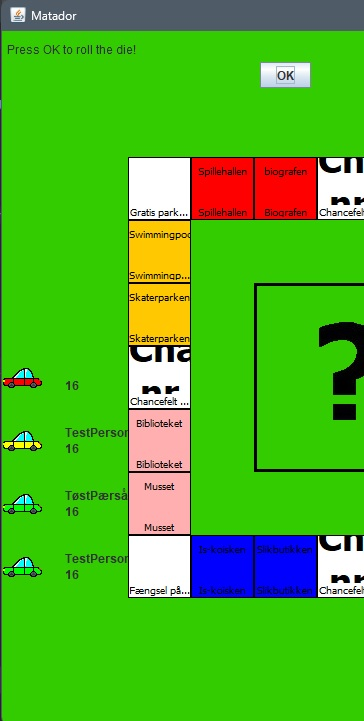
\includegraphics[height = 10cm]{Billeder/TC01.jpg}\\
    \hline
    Status & Gennemført.\\
    \hline
    Tested by & Jakob Agergaard\\
    \hline
    Date & 18-11-2022\\
    \hline
    Test environment & IntelliJ IDEA 2022.2.3 (Ultimate Edition)\\
      & Build \#IU-222.4345.14, built on October 5, 2022\\
      & on Windows 11 Home version 22H2\\
    \hline
\end{tabular}
\subsection{Test case 02}
\begin{tabular}{ | m{0.2\textwidth} | m{0.8\textwidth}|}
    \hline
    Test case ID & TC02  \\
    \hline
    Summary & Tester om spillerne kan udføre en tur\\
    \hline
    Requirements & Tester ift. krav 3, 6 og 7.\\
    \hline
    Preconditions & Bruger har indtastet antal spillere og navne.\\
    \hline
    Postconditions & Turen gives videre til næste spiller (loop fortsætter)\\
    \hline
    Test Procedure & \begin{enumerate}[itemsep=0.1mm]
        \item Tryk enter/OK for at slå med terningen
        \item Tryk enter/OK for at flytte brikken
        \item Tryk enter/OK for at anerkende besked fra system
        \item Tryk enter/OK for at give turen videre
        \item Gentag ovenstående mindst 4 gange
    \end{enumerate}\\
    \hline
    Test data & Manuelt input gennem GUI (Tryk OK, for at spillet går til næste stadie)\\
    \hline
    Expected result & Systemet kører spillerens tur igennem og meddeler derefter hvilken spiller der nu skal til at tage sin tur.\\
    \hline
    Actual result & Der opstår en NullPointerError i linje 78 Der forsøger at opdatere spillerens balance i GUI'en. Den samme fejl vil formentlig også vise sig i linje 79.\\
     & 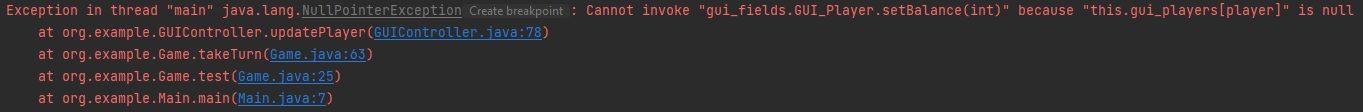
\includegraphics[width = 0.8\textwidth]{Billeder/TC02-1.jpg}\\
     & 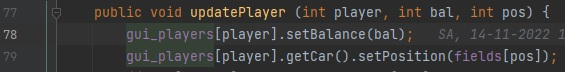
\includegraphics[width = 0.6\textwidth]{Billeder/TC02-2.jpg}\\
     & Ved nærmere undersøgelse fandt vi ud af hvorfor dette skete. Grunden findes i metoden der opretter netop gui\_players arrayet.\\
     & 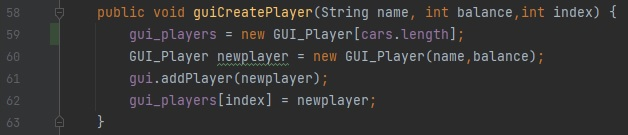
\includegraphics[width = 0.6\textwidth]{Billeder/TC02-3.jpg}\\
     & Løsningen på dette blev at lade dette array blive oprettet allerede umiddelbart efter spillernes brikker er blevet oprettet\\
     & 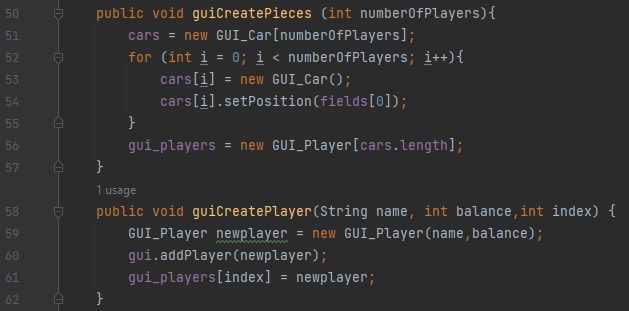
\includegraphics[width = 0.6\textwidth]{Billeder/TC02-4.jpg}\\
    \hline
    Status & Først fejlet.\\
     & Efterfølgende fikset og gennemført.\\
    \hline
    Tested by & Jakob Agergaard\\
    \hline
    Date & 18-11-2022\\
    \hline
    Test environment & IntelliJ IDEA 2022.2.3 (Ultimate Edition)\\
      & Build \#IU-222.4345.14, built on October 5, 2022\\
      & on windows 11 Home version 22H2\\
    \hline
\end{tabular}
sfadfasfsda\\
\begin{tabular}{ | m{0.2\textwidth} | m{0.8\textwidth}|}
    \hline
    Test case ID & TC03  \\
    \hline
    Summary & \\
    \hline
    Requirements & \\
    \hline
    Preconditions & \\
    \hline
    Postconditions & \\
    \hline
    Test Procedure & \\
    \hline
    Test data &  \\
    \hline
    Expected result & \\
    \hline
    Actual result & \\
    \hline
    Status & \\
    \hline
    Tested by & \\
    \hline
    Date & \\
    \hline
    Test environment & \\
    \hline
\end{tabular}

\section{Bugfixes}
I implementeringen af chancekortene, stødte vi på et problem der gjorde at, når der landes på et chancefelt, så vises ét chancekort, men handlingerne for et andet chancekort bliver udført.\\
Årsagen til dette var at der, når man lander på et chancekort, bliver valgt tilfældigt mellem tre mulige chancekort-handlinger, og denne bliver derefter udført. På samme måde blev tekst for chancekortet (displayChanceCard(txt)), også valgt tilfældigt mellem tre mulige chancekort-handlinger. \\
Disse var altså uafhængige af hinanden, og derfor opstod problemet.
Løsninge til dette var...

Et bug, hvis samme navn er indtastet gælder det kun som en spiller.


\section{Konklusion}
På baggrund af ovenstående rapport, kan man se at der er blevet produceret en use case, en række diagrammere og programmeret Monopoly Junior, som indeholder kundens vision og alle kravene som hertil følger. Ud fra en analyse er der blevet lavet en use casen og fremstillet nogle diagrammerne, og de er vigtig for dette projekt, da de
er det grundlæggende for hele opgaven. Diagrammerne er dem som simplificere programmet, som i sidste ende gør opgaven at programmere et Monopoly Junior spil mere overskueligt og derfor også nemmere. Den bruger venlige test sikre os, at det programmeret Monopoly Junior spil kan spilles af mennesker, som ikke har været en del af dette projekt eller anden relation. Der kan derfor konkluderes at der er blevet produceret et Monopoly  Junior spil efter kundens ønske, hvilket tager udgangspunkt i deres vision og krav, samt egen vurdering af hvad Monopoly Junior spillet skal indeholde.  
\section{Bilag}
\subsection{Litteratur}
\subsection{Kode}

\end{document}